%%%%%%%%%%%%%%%%%%%%%%%%%%%%%%%%%%%%%%%%%%%%%%%%%%%%%%%%%%%%%%%%%%%%%%%%%%%

\documentclass[a4paper,oneside,12pt]{article}
\usepackage{mystyle}

\begin{document}

\title{\Large\bf Cartesian coordinate system}
\author{%%
  Minh Van Nguyen \\
  \url{mvngu@gmx.com}
}
\date{\today}
\maketitle


%%%%%%%%%%%%%%%%%%%%%%%%%%%%%%%%%%%%%%%%%%%%%%%%%%%%%%%%%%%%%%%%%%%%%%%%%%%

\section{Coordinates}

Let's start by discussing how a pair of numbers can be represented as
a picture.  You know that any real number can be represented as a
point on the number line.  \Figure{fig:real_number_line} shows the
irrational numbers $\sqrt{2}$, $e$, and $\pi$ as points on the number
line.  What if you have a pair $\tuple{a}{b}$ of real numbers?  How
would $\tuple{a}{b}$ be represented as a point on the number line?

\begin{figure}[!htbp]
\centering
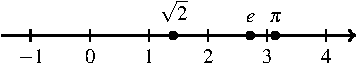
\includegraphics[scale=1.1]{image/03/number-line.pdf}
\caption{%%
  Elements from the set $\RR$ of real numbers can be represented as
  points on the number line.
}
\label{fig:real_number_line}
\end{figure}

The answer is that a pair $\tuple{a}{b}$ of real numbers cannot be
represented as a point on the number line.  You must somehow extend
the number line.  One way to extend the number line is to draw a
vertical line through the point $0$ such that the vertical line is
perpendicular to the number line.  What you then obtain is the
\emph{Cartesian coordinate system} as shown in
\Figure{fig:Cartesian_coordinate_system}.  In the Cartesian coordinate
system, a pair $\tuple{a}{b}$ of real numbers can be represented as a
point.  The pair $\tuple{a}{b}$ is now called a pair of
\emph{coordinates}.  The number $a$ in the coordinates $\tuple{a}{b}$
is called the $x$-coordinate because starting from $0$ on the
$x$-axis you must move a horizontal distance of $a$ units to get to
the coordinates $\tuple{a}{0}$.  The number $b$ in the coordinates
$\tuple{a}{b}$ is called the $y$-coordinate because starting from $0$
on the $y$-axis you must move a vertical distance of $b$ units to get
to the coordinates $\tuple{0}{b}$.  Add the coordinates $\tuple{a}{0}$
and $\tuple{0}{b}$ together and you get the coordinates
$\tuple{a}{b}$, which can be drawn as a point in the Cartesian
coordinate system.  The special coordinates $\tuple{0}{0}$ is called
the \emph{origin}.  If $\tuple{a}{b}$ is a pair of coordinates in the
Cartesian coordinate system, you also refer to $\tuple{a}{b}$ as a
point in the Cartesian coordinate system.

\begin{figure}[!htbp]
\centering
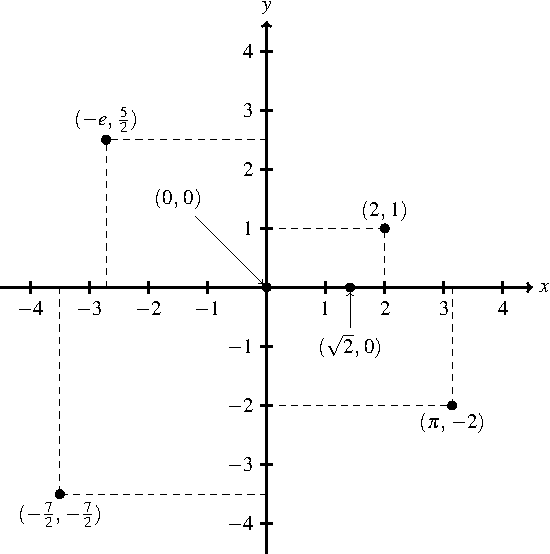
\includegraphics[scale=1.1]{image/03/cartesian-coordinate.pdf}
\caption{%%
  The Cartesian coordinate system consists of two perpendicular axes
  called the $x$-axis and the $y$-axis.  A pair $\tuple{a}{b}$ of real
  numbers can be represented as a point.  Starting from the origin
  $\tuple{0}{0}$, you move a distance of $a$ units along the
  horizontal axis and then move $b$ units along the vertical axis.
  Where you end up is the point $\tuple{a}{b}$.
}
\label{fig:Cartesian_coordinate_system}
\end{figure}

\begin{exercise}
Represent the pairs $\tuple{2}{4}$, $\tuple{0}{-3}$, and
$\tuple{-4}{0}$ as points in the Cartesian coordinate system.
\end{exercise}

\ifbool{showSolution}{
\begin{solution}
See \Figure{fig:some_points_in_Cartesian_coordinate_system}.
%%
\begin{figure}[!htbp]
\centering
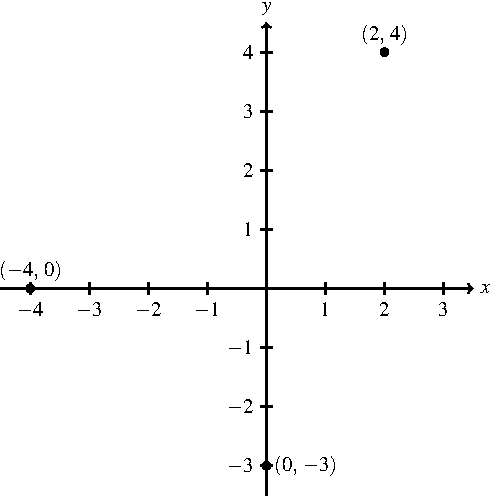
\includegraphics[scale=1.1]{image/03/cartesian-coordinate_2-5_0-3_4-0.pdf}
\caption{%%
  The pairs $\tuple{2}{4}$, $\tuple{0}{-3}$, and $\tuple{-4}{0}$ as
  points in the Cartesian coordinate system.
}
\label{fig:some_points_in_Cartesian_coordinate_system}
\end{figure}
\end{solution}
}{}


%%%%%%%%%%%%%%%%%%%%%%%%%%%%%%%%%%%%%%%%%%%%%%%%%%%%%%%%%%%%%%%%%%%%%%%%%%%

\section{Distance}

The distance between two points $A$ and $B$ is the length of the
straight line from $A$ to $B$.  In the Cartesian coordinate system,
you use the same technique to measure the distance between two
points.  Suppose the points $A$ and $B$ have coordinates
$A = \tuple{x_1}{y_1}$ and $B = \tuple{x_2}{y_2}$; see
\Figure{fig:distance_between_two_points}.  Then there is a third point
$C$ with coordinates $C = \tuple{x_1}{y_2}$.  The line segments $AC$,
$BC$, and $AB$ are the three sides of a right-angled triangle.  The
vertical segment $AC$ has length
\[
a
=
\absoluteValue{y_1 - y_2}
=
\absoluteValue{y_2 - y_1}.
\]
Recall that if $x$ is any number, then its absolute value is denoted
$\absoluteValue{x}$ and defined by
\[
\absoluteValue{x}
=
\begin{cases}
x, & \text{if $x \geq 0$}, \\[4pt]
-x, & \text{if $x < 0$}.
\end{cases}
\]
The vertical segment $AC$ is also called the
\emph{change in the vertical direction}.  The horizontal segment $BC$
has length
\[
b
=
\absoluteValue{x_2 - x_1}
=
\absoluteValue{x_1 - x_2}.
\]
The horizontal segment $BC$ is also called the
\emph{change in the horizontal direction}.  However, you do not yet
know the length of the hypotenuse $AB$.  Since the points
$\triple{A}{B}{C}$ are the three corners of a right-angled triangle,
you can use Pythagoras' theorem to determine the length of the
hypotenuse $AB$.

\begin{figure}[!htbp]
\centering
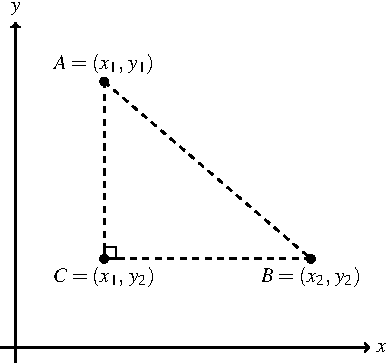
\includegraphics[scale=1.1]{image/03/distance-two-points.pdf}
\caption{%%
  Any two points $\pair{A}{B}$ are corners of a right-angled triangle.
  The segment $AB$ is the hypotenuse, whose length can be measured by
  Pythagoras' theorem.
}
\label{fig:distance_between_two_points}
\end{figure}

\begin{theorem}
\textbf{Pythagoras' theorem.}
Let $\triple{a}{b}{c}$ be the lengths of the three sides of a
right-angled triangle, where $c$ is the length of the hypotenuse.
Then $c$ can be written as $a^2 + b^2 = c^2$.
\end{theorem}

\begin{figure}[!htbp]
\centering
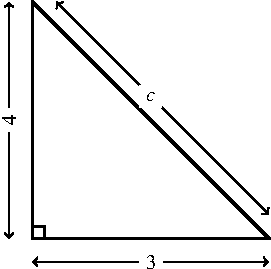
\includegraphics[scale=1.1]{image/03/345-triangle.pdf}
\caption{%%
  A right-angled triangle whose base and height are $3$ and $4$ units,
  respectively.  The value of the hypotenuse is denoted $c$.
}
\label{fig:345_triangle}
\end{figure}

\begin{example}
\Figure{fig:345_triangle} shows a right-angled triangle whose
hypotenuse is unknown.  Calculate the length of the hypotenuse.
\end{example}

\begin{solution}
Let $a = 3$ be the length of the base of the triangle, $b = 4$ be the
height of the triangle, and $c$ the hypotenuse.  Using Pythagoras'
theorem, you have the equation
%%
\begin{align*}
c^2
&=
3^2 + 4^2 \\[4pt]
&=
9 + 16 \\[4pt]
&=
25.
\end{align*}
%%
Solving the last equation for $c$ shows that $c = \sqrt{25} = 5$.
Therefore for the right-angled triangle in \Figure{fig:345_triangle}
the hypotenuse has a length of $c = 5$ units.
\end{solution}

\begin{figure}[!htbp]
\centering
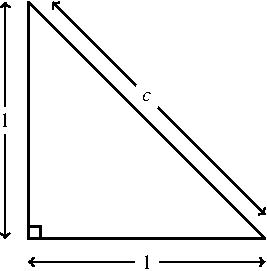
\includegraphics[scale=1.1]{image/03/triangle.pdf}
\caption{%%
  A right-angled triangle each of whose base and height is one unit.
  The value of the hypotenuse is denoted $c$.
}
\label{fig:right_angled_triangle}
\end{figure}

\begin{exercise}
Consider the right-angled triangle in
\Figure{fig:right_angled_triangle}.  Suppose that each of the
triangle's base and height is one unit.  Compute the value of the
hypotenuse.
\end{exercise}
\ifbool{showSolution}{
  \begin{solution}
  Use Pythagoras' theorem to write the value of the hypotenuse $c$ as
  %%
  \begin{align*}
  c^2
  &=
  1^2 + 1^2 \\[4pt]
  &=
  2.
  \end{align*}
  %%
  Solve the last equation for $c$ to get $c = \sqrt{2}$.
  \end{solution}
}{}

\begin{exercise}
\begin{packedenum}
\item\label{subex:absolute_value_4_minus_5}
  Show that the absolute value $\absoluteValue{4 - 5}$ is the same as
  the absolute value $\absoluteValue{5 - 4}$.

\item\label{subex:absolute_value_7_minus_3}
  Show that $\absoluteValue{7 - 3} = \absoluteValue{3 - 7}$.

\item\label{subex:absolute_value_a_minus_b}
  Let $a$ and $b$ be any numbers.  Explain why
  $\absoluteValue{a - b} = \absoluteValue{b - a}$.
\end{packedenum}
\end{exercise}

\ifbool{showSolution}{
\begin{solution}
\solutionpart{subex:absolute_value_4_minus_5}
You have $\absoluteValue{4 - 5} = \absoluteValue{-1} = 1$ and
$\absoluteValue{5 - 4} = \absoluteValue{1} = 1$.  Therefore you have
the equality
$\absoluteValue{4 - 5} = \absoluteValue{5 - 4}$.

\solutionpart{subex:absolute_value_7_minus_3}
The solution is similar to \Part{subex:absolute_value_4_minus_5}.  You
have the absolute value
$\absoluteValue{7 - 3} = \absoluteValue{4} = 4$ and
$\absoluteValue{3 - 7} = \absoluteValue{-4} = 4$.  Therefore you have
$\absoluteValue{7 - 3} = \absoluteValue{3 - 7}$.

\solutionpart{subex:absolute_value_a_minus_b}
The numbers $a$ and $b$ can be represented as the points
$\tuple{a}{0}$ and $\tuple{b}{0}$, respectively, in the Cartesian
coordinate system.  The absolute value $\absoluteValue{a - b}$ is the
distance between the points $\tuple{a}{0}$ and $\tuple{b}{0}$.  Since
$\absoluteValue{b - a}$ is also the distance between $\tuple{a}{0}$
and $\tuple{b}{0}$, it follows that
$\absoluteValue{a - b} = \absoluteValue{b - a}$.
\end{solution}
}{}

\begin{exercise}
\label{ex:absolute_value_squared}
\begin{packedenum}
\item\label{subex:absolute_value_squared_4_minus_5}
  Show that $\absoluteValue{4 - 5}^2$ is the same as $(4 - 5)^2$.

\item\label{subex:absolute_value_squared_7_minus_3}
  Show that $\absoluteValue{7 - 3}^2$ is the same as $(7 - 3)^2$.

\item\label{subex:absolute_value_squared_a_minus_b}
  Let $a$ and $b$ be any numbers.  Explain why
  $\absoluteValue{a - b}^2 = (a - b)^2$.
\end{packedenum}
\end{exercise}

\ifbool{showSolution}{
\begin{solution}
\solutionpart{subex:absolute_value_squared_4_minus_5}
The absolute value $\absoluteValue{4 - 5}^2$ can be written as
%%
\begin{align*}
\absoluteValue{4 - 5}^2
&=
\absoluteValue{-1}^2 \\[4pt]
&=
\absoluteValue{-1} \times \absoluteValue{-1} \\[4pt]
&=
1 \times 1 \\[4pt]
&=
1^2 \\[4pt]
&=
1.
\end{align*}
%%
Furthermore, you have $(4 - 5)^2 = (-1)^2 = 1$ and therefore
$\absoluteValue{4 - 5}^2 = (4 - 5)^2$.

\solutionpart{subex:absolute_value_squared_7_minus_3}
You can write $\absoluteValue{7 - 3}^2$ as
%%
\begin{align*}
\absoluteValue{7 - 3}^2
&=
\absoluteValue{-4}^2 \\[4pt]
&=
\absoluteValue{-4} \times \absoluteValue{-4} \\[4pt]
&=
4 \times 4 \\[4pt]
&=
16.
\end{align*}
%%
Furthermore, you can write
$(7 - 3)^2 = (-4)^2 = (-1)^2 \times 4^2 = 16$ and therefore you have
$\absoluteValue{7 - 3}^2 = (7 - 3)^2$.

\solutionpart{subex:absolute_value_squared_a_minus_b}
Since $a$ and $b$ are any numbers, you have three cases:
%%
\begin{packedenumeral}
\item\label{case:a_less_than_b}
  $a < b$,

\item\label{case:a_equals_b}
  $a = b$,

\item\label{case:a_greater_than_b}
  $a > b$.
\end{packedenumeral}
%%
Note that
$\absoluteValue{a - b}^2
=
\absoluteValue{a - b} \times \absoluteValue{a - b}$ and
$(a - b)^2 = (a - b) (a - b)$.  Let's consider the above cases in
turn.

\solutionpart{case:a_less_than_b}
Suppose $a < b$.  Then $a - b < 0$ and from the definition of absolute
value you have $a - b = -\absoluteValue{a - b}$.  You can write
$(a - b)^2$ as
%%
\begin{align*}
(a - b)^2
&=
\bigparen{
  -\absoluteValue{a - b}
}^2 \\[4pt]
&=
\bigparen{
  -\absoluteValue{a - b}
}
\times
\bigparen{
  -\absoluteValue{a - b}
} \\[4pt]
&=
(-1) \times (-1)
\times
\absoluteValue{a - b} \times \absoluteValue{a - b} \\[4pt]
&=
\absoluteValue{a - b}^2.
\end{align*}

\solutionpart{case:a_equals_b}
If $a = b$, then $a - b = 0$ and so you have
$\absoluteValue{a - b}^2 = 0^2 = (a - b)^2$.

\solutionpart{case:a_greater_than_b}
Assume that $a > b$.  Then $a - b > 0$ and the absolute value of
$a - b$ can be written as $\absoluteValue{a - b} = a - b$.  Square
both sides of the latter equation to obtain
$\absoluteValue{a - b}^2 = (a - b)^2$.

In all of the above cases, you have
$\absoluteValue{a - b}^2 = (a - b)^2$ no matter what the values of
$a$ and $b$ are.
\end{solution}
}{}

Let $c$ be the length of the hypotenuse $AB$ in
\Figure{fig:distance_between_two_points}.  Use Pythagoras' theorem and
\Exercise{ex:absolute_value_squared} to write
%%
\begin{align*}
c^2
&=
a^2 + b^2 \\[4pt]
&=
\absoluteValue{y_2 - y_1}^2 + \absoluteValue{x_2 - x_1}^2 \\[4pt]
&=
(y_2 - y_1)^2 + (x_2 - x_1)^2.
\end{align*}
%%
Solve the last expression for $c$ and you obtain
\[
c
=
\sqrt{
  (y_2 - y_1)^2
  +
  (x_2 - x_1)^2
}
\]
which proves the following theorem.

\begin{theorem}
\label{thm:distance_between_two_points}
\textbf{Distance.}
Let $A = \tuple{x_1}{y_1}$ and $B = \tuple{x_2}{y_2}$ be two points in
the Cartesian coordinate system.  The distance between $A$ and $B$ can
be written as
\[
\sqrt{
  (y_2 - y_1)^2
  +
  (x_2 - x_1)^2
}.
\]
\end{theorem}

\begin{example}
Consider the points $(\sqrt{2}\comma 0)$ and $\tuple{2}{1}$ from
\Figure{fig:Cartesian_coordinate_system}.  Determine the distance
between those two points.
\end{example}

\begin{solution}
Use \Theorem{thm:distance_between_two_points} to write
%%
\begin{align*}
\sqrt{
  (1 - 0)^2
  +
  (2 - \sqrt{2})^2
}
&=
\sqrt{
  1^2 + (2 - \sqrt{2})^2
} \\[4pt]
&\approx
1.3431
\end{align*}
%%
correct to four decimal places.  The symbol ``$\approx$'' means
``approximately''.  In other words, the distance between the points
$(\sqrt{2}\comma 0)$ and $\tuple{2}{1}$ is approximately $1.3431$.
\end{solution}

\begin{exercise}
Calculate the distance from the point $\tuple{0}{3}$ to the origin.
Determine the distance from the point $\tuple{0}{-3}$ to the origin.
\end{exercise}

\ifbool{showSolution}{
\begin{solution}
The distance from the point $\tuple{0}{3}$ to the origin is
%%
\begin{align*}
\sqrt{
  (3 - 0)^2 + (0 - 0)^2
}
&=
\sqrt{3^2} \\[4pt]
&=
3.
\end{align*}
%%
The distance from the point $\tuple{0}{-3}$ to the origin is
%%
\begin{align*}
\sqrt{
  (-3 - 0)^2 + (0 - 0)^2
}
&=
\sqrt{(-3)^2} \\[4pt]
&=
\sqrt{(-1)^2 \times 3^2} \\[4pt]
&=
\sqrt{3^2} \\[4pt]
&=
3.
\end{align*}
\end{solution}
}{}

\begin{exercise}
Let $\tuple{a}{b}$ be any point in the Cartesian coordinate system.
Calculate the distance from $\tuple{a}{b}$ to the origin.
\end{exercise}

\ifbool{showSolution}{
\begin{solution}
Use \Theorem{thm:distance_between_two_points} to write
%%
\begin{align*}
\sqrt{
  (a - 0)^2 + (b - 0)^2
}
&=
\sqrt{
  a^2 + b^2
}
\end{align*}
%%
which is the distance from the origin to $\tuple{a}{b}$.
\end{solution}
}{}

\begin{exercise}
\label{ex:distance_from_point_to_itself_is_zero}
If $A = \tuple{a}{b}$ is any point in the Cartesian coordinate system,
explain why the distance from $A$ to itself is zero.
\end{exercise}

\ifbool{showSolution}{
\begin{solution}
\Theorem{thm:distance_between_two_points} does not assume that any two
points must be distinct in order to compute the distance between the
points.  You can use \Theorem{thm:distance_between_two_points} to
write
%%
\begin{align*}
\sqrt{
  (b - b)^2 + (a - a)^2
}
&=
\sqrt{
  0^2 + 0^2
} \\[4pt]
&=
\sqrt{0} \\[4pt]
&=
0
\end{align*}
%%
which shows that the distance from any point to itself is zero.
\end{solution}
}{}

\begin{exercise}
  Suppose $a \geq 0$ is a real number.  Let $A$ be the distance
  from the point $\tuple{a}{0}$ to the origin, let $B$ be the distance
  from the point $\tuple{-a}{0}$ to the origin, $C$ the distance from
  $\tuple{0}{a}$ to the origin, and $D$ the distance from
  $\tuple{0}{-a}$ to the origin.  Explain why $A = B = C = D$.
\end{exercise}

\ifbool{showSolution}{
\begin{solution}
The four points $\tuple{a}{0}$, $\tuple{-a}{0}$, $\tuple{0}{a}$, and
$\tuple{0}{-a}$ lie on a circle of radius $a$, where the circle is
centred at the origin; see \Figure{fig:four_points_on_a_circle}.
Therefore each of the points is the same distance from the origin.  On
the other hand, you can use \Theorem{thm:distance_between_two_points}
to calculate the distances.  The distance $A$ is
\[
A
=
\sqrt{
  (0 - 0)^2 + (a - 0)^2
}
=
\sqrt{a^2}.
\]
The distance $B$ is
\[
B
=
\sqrt{
  (0 - 0)^2 + (-a - 0)^2
}
=
\sqrt{(-a)^2}
=
\sqrt{a^2}.
\]
The distance $C$ is
\[
C
=
\sqrt{
  (a - 0)^2 + (0 - 0)^2
}
=
\sqrt{a^2}.
\]
The distance $D$ is
\[
D
=
\sqrt{
  (-a - 0)^2 + (0 - 0)^2
}
=
\sqrt{(-a)^2}
=
\sqrt{a^2}.
\]
Since $a \geq 0$, each of the above distances simplify to $a$ and
therefore $A = B = C = D$.

\begin{figure}[!htbp]
\centering
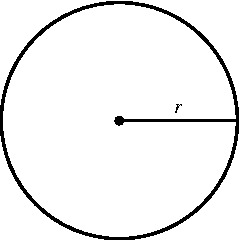
\includegraphics[scale=1.1]{image/03/circle.pdf}
\caption{%%
  A circle of radius $a \geq 0$ and centred at the origin
  $\tuple{0}{0}$.
}
\label{fig:four_points_on_a_circle}
\end{figure}
\end{solution}
}{}


%%%%%%%%%%%%%%%%%%%%%%%%%%%%%%%%%%%%%%%%%%%%%%%%%%%%%%%%%%%%%%%%%%%%%%%%%%%

\section{Reflection}

Let $\tuple{a}{b}$ be any point in the Cartesian coordinate system.
You can do a number of basic geometric operations on $\tuple{a}{b}$ by
multiplying $a$ or $b$ by $-1$.  For example, imagine you place a
mirror along the $x$-axis.  Then the reflection of $\tuple{a}{b}$ with
respect to the $x$-axis is $\tuple{a}{-1 \times b} = \tuple{a}{-b}$.
If you now place a mirror along the $y$-axis, the reflection of
$\tuple{a}{b}$ with respect to the $y$-axis is
$\tuple{-1 \times a}{b} = \tuple{-a}{b}$.  Multiplying each of $a$ and
$b$ by $-1$ and you get $\tuple{-a}{-b}$, which is the diagonal
reflection of $\tuple{a}{b}$.  See \Figure{fig:reflections_of_point}
for an example.

\begin{figure}[!htbp]
\centering
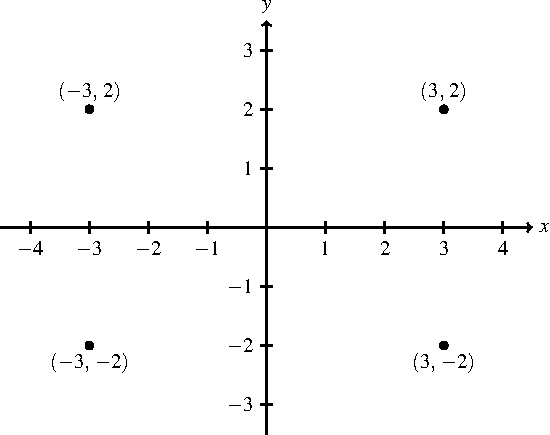
\includegraphics[scale=1.1]{image/03/reflection.pdf}
\caption{%%
  Some reflections of the point $A = \tuple{3}{2}$.  The point
  $\tuple{3}{-2}$ is the reflection of $A$ with respect to the
  $x$-axis.  The point $\tuple{-3}{2}$ is the reflection of $A$ with
  respect to the $y$-axis.  The diagonal reflection of $A$ is the
  point $\tuple{-3}{-2}$.  The point $A$ together with its three
  reflections form the four corners of a rectangle.  The centre of the
  rectangle is the origin $\tuple{0}{0}$.
}
\label{fig:reflections_of_point}
\end{figure}

\begin{example}
Consider the point $A = \tuple{1}{2}$.
%%
\begin{packedenum}
\item\label{subex:point_1_2_reflection_x_axis}
  Determine the reflection of $A$ with respect to the $x$-axis.

\item\label{subex:point_1_2_reflection_y_axis}
  Determine the reflection of $A$ with respect to the $y$-axis.

\item\label{subex:point_1_2_reflection_diagonal}
  Determine the diagonal reflection of $A$.
\end{packedenum}
\end{example}

\begin{solution}
\solutionpart{subex:point_1_2_reflection_x_axis}
The reflection of $A$ with respect to the $x$-axis is obtained by
multiplying the $y$-coordinate by $-1$.  Thus
\[
\tuple{1}{-1 \times 2}
=
\tuple{1}{-2}
\]
is the reflection of $A$ with respect to the $x$-axis.

\solutionpart{subex:point_1_2_reflection_y_axis}
You can calculate the reflection of $A$ with respect to the $y$-axis
by multiplying the $x$-coordinate by $-1$.  Thus
\[
\tuple{-1 \times 1}{2}
=
\tuple{-1}{2}
\]
is the reflection of $A$ with respect to the $y$-axis.

\solutionpart{subex:point_1_2_reflection_diagonal}
The diagonal reflection of $A$ is obtained by multiplying each of the
coordinates by $-1$.  Thus
\[
\tuple{-1 \times 1}{-1 \times 2}
=
\tuple{-1}{-2}
\]
is the diagonal reflection of $A$.
\end{solution}

\begin{exercise}
Consider the point $A = \tuple{-2}{4}$.  Determine the reflections of
$A$ with respect to the $x$- and $y$-axes and also the diagonal
reflection of $A$.
\end{exercise}

\ifbool{showSolution}{
\begin{solution}
See \Figure{fig:reflections_of_m2_4}.  The reflection of $A$ with
respect to the $x$-axis is $\tuple{-2}{-4}$.  The reflection of $A$
with respect to the $y$-axis is $\tuple{2}{4}$.  The diagonal
reflection is $\tuple{2}{-4}$.
%%
\begin{figure}[!htbp]
\centering
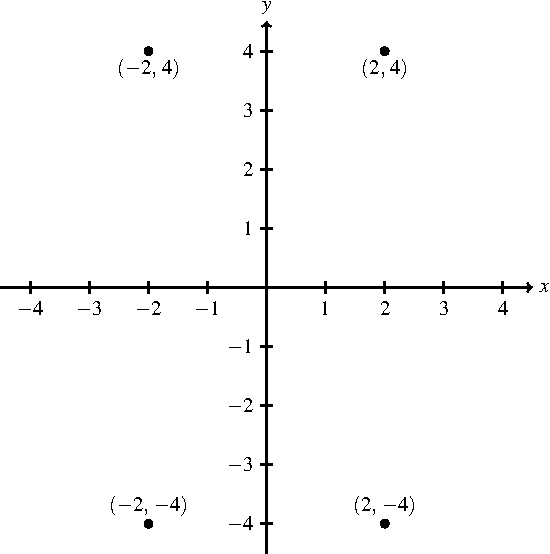
\includegraphics[scale=1.1]{image/03/reflection-eg.pdf}
\caption{%%
  Reflections of the point $\tuple{-2}{4}$.
}
\label{fig:reflections_of_m2_4}
\end{figure}
\end{solution}
}{}


\newpage
%%%%%%%%%%%%%%%%%%%%%%%%%%%%%%%%%%%%%%%%%%%%%%%%%%%%%%%%%%%%%%%%%%%%%%%%%%%

\section*{Problem}

\begin{problem}
\item Ren\'e Descartes is credited with inventing the Cartesian
  coordinate system.  Read more about Descartes at Wikipedia and the
  MacTutor History of Mathematics archive:
  %%
  \begin{center}
  \url{http://www-groups.dcs.st-and.ac.uk/~history/}
  \end{center}
  %%
  Search for ``Ren\'e Descartes''.

\item This problem tests your understanding of absolute value and
  distance.
  %%
  \begin{packedenum}
  \item\label{subprob:point_on_axis_to_origin_2}
    Show that the distance from the point $\tuple{2}{0}$ to the origin
    is the absolute value $\absoluteValue{2}$.

  \item\label{subprob:point_on_axis_to_origin_minus_3}
    Show that the distance from the point $\tuple{-3}{0}$ to the
    origin is the absolute value $\absoluteValue{-3}$.

  \item\label{subprob:point_on_axis_to_origin_general}
    Let $a$ be a real number.  Explain why the distance from the point
    $\tuple{a}{0}$ to the origin is the absolute value
    $\absoluteValue{a}$.
  \end{packedenum}
\ifbool{showSolution}{
  \begin{solution}
  \solutionpart{subprob:point_on_axis_to_origin_2}
  From the origin $\tuple{0}{0}$ you travel a distance of $2$ units to
  the right in order to reach the point $\tuple{2}{0}$.  Thus the
  distance between the points $\tuple{0}{0}$ and $\tuple{2}{0}$ is
  $\absoluteValue{2} = 2$.

  \solutionpart{subprob:point_on_axis_to_origin_minus_3}
  Starting from the origin $\tuple{0}{0}$ you travel a distance of $3$
  units to the left in order to reach the point $\tuple{-3}{0}$.  Thus
  the distance between the points $\tuple{0}{0}$ and $\tuple{-3}{0}$
  is $\absoluteValue{-3} = 3$.

  \solutionpart{subprob:point_on_axis_to_origin_general}
  You have three cases: (1)~$a > 0$, (2)~$a < 0$, and (3)~$a = 0$.  If
  $a > 0$, then the point $\tuple{a}{0}$ is to the right of the origin
  $\tuple{0}{0}$.  Starting from the origin, you travel a distance of
  $a$ units to the right to reach the point $\tuple{a}{0}$.  Note that
  $\absoluteValue{a} = a$ because you assumed that $a > 0$.

  If $a < 0$, then the point $\tuple{a}{0}$ is to the left of the
  origin $\tuple{0}{0}$.  Starting from the origin, you travel a
  distance of $\absoluteValue{a}$ units to the left in order to reach
  the point $\tuple{a}{0}$.  Since you assumed that $a < 0$, then the
  absolute value $\absoluteValue{a} = -a$.  Thus the point
  $\tuple{a}{0}$ has a distance of $\absoluteValue{a}$ to the origin.

  If $a = 0$, then from
  \Exercise{ex:distance_from_point_to_itself_is_zero} you know that
  the distance from $\tuple{0}{0}$ to itself is zero.  Note that
  $\absoluteValue{0} = 0$.  In each of the above three cases, you have
  a distance of $\absoluteValue{a}$ from $\tuple{a}{0}$ to the
  origin.
  \end{solution}
}{}

\item Let $a$ and $b$ be positive numbers such that $a \leq b$.
  Suppose you have two points $A = \tuple{a}{0}$ and
  $B = \tuple{b}{0}$.  If you now have a point $C$ defined by
  \[
  C
  =
  \tuple{
    \frac{a + b}{2}
  }{
    0
  }
  \]
  explain why $C$ is midway between $A$ and $B$.
\ifbool{showSolution}{
  \begin{solution}
  Let $d$ be the distance between $A$ and $B$.  The distance midway
  between $A$ and $B$ is $d/2$.  Then the point
  $\tuple{a + \frac{d}{2}}{0}$ is midway between $A$ and $B$.  Let's
  verify that the above is true for the point $C$.  Use
  \Theorem{thm:distance_between_two_points} to get
  %%
  \begin{align*}
  d
  &=
  \sqrt{
    (0 - 0)^2 + (b - a)^2
  } \\[4pt]
  &=
  \sqrt{(b - a)^2}.
  \end{align*}
  %%
  Since $a$ and $b$ are positive with $a \leq b$, then the difference
  $b - a$ satisfies $b - a \geq 0$.  In other words, the distance
  between $A$ and $B$ can be written as $d = b - a$.  The expression
  $a + \frac{d}{2}$ can be written as
  %%
  \begin{align*}
  a + \frac{d}{2}
  &=
  a + \frac{b - a}{2} \\[4pt]
  &=
  \frac{2a}{2}
  +
  \frac{b - a}{2} \\[4pt]
  &=
  \frac{2a + b - a}{2} \\[4pt]
  &=
  \frac{a + b}{2}
  \end{align*}
  %%
  which is the $x$-coordinate of the point $C$.  Therefore $C$ is the
  point midway between $A$ and $B$.
  \end{solution}
}{}

\item Let $a$ and $b$ be positive numbers such that $a \leq b$.
  Suppose you have two points $A = \tuple{a}{0}$ and
  $B = \tuple{b}{0}$, where the segment $L$ is the straight line that
  starts from $A$ and ends at $B$.  You break up the segment $L$ into
  four pieces of equal length.  Determine the start and end
  coordinates of each of the four pieces.
\ifbool{showSolution}{
  \begin{solution}
  The distance between $A$ and $B$ is $b - a \geq 0$.  If the line
  segment $L$ is broken up into four pieces of equal length, then each
  piece will have a length of $\ell = \frac{b - a}{4}$.  The first
  piece ends at the coordinates $\tuple{a + \ell}{0}$, where
  $a + \ell$ can be written as
  %%
  \begin{align*}
  a + \ell
  &=
  a + \frac{b - a}{4} \\[4pt]
  &=
  \frac{4a}{4} + \frac{b - a}{4} \\[4pt]
  &=
  \frac{
    4a + b - a
  }{
    4
  } \\[4pt]
  &=
  \frac{
    3a + b
  }{
    4
  }.
  \end{align*}
  %%
  In other words, the first piece has coordinates from $\tuple{a}{0}$
  to $\tuple{\frac{3a + b}{4}}{0}$.  The second piece ends at the
  coordinates $\tuple{a + 2\ell}{0}$, where $a + 2\ell$ can be written
  as
  %%
  \begin{align*}
  a + 2\ell
  &=
  a + 2 \times \frac{b - a}{4} \\[4pt]
  &=
  a + \frac{b - a}{2} \\[4pt]
  &=
  \frac{2a}{2} + \frac{b - a}{2} \\[4pt]
  &=
  \frac{
    2a + b - a
  }{
    2
  } \\[4pt]
  &=
  \frac{
    a + b
  }{
    2
  }.
  \end{align*}
  %%
  Then the second piece has coordinates from
  $\tuple{\frac{3a + b}{4}}{0}$ to $\tuple{\frac{a + b}{2}}{0}$.  The
  third piece ends at the coordinates $\tuple{a + 3\ell}{0}$, where
  $a + 3\ell$ can be written as
  %%
  \begin{align*}
  a + 3\ell
  &=
  a + 3 \times \frac{b - a}{4} \\[4pt]
  &=
  a + \frac{3(b - a)}{4} \\[4pt]
  &=
  \frac{4a}{4} + \frac{3b - 3a}{4} \\[4pt]
  &=
  \frac{
    4a + 3b - 3a
  }{
    4
  } \\[4pt]
  &=
  \frac{
    a + 3b
  }{
    4
  }.
  \end{align*}
  %%
  So the third piece has coordinates from $\tuple{\frac{a + b}{2}}{0}$
  to $\tuple{\frac{a + 3b}{4}}{0}$.  Finally, the fourth piece ends at
  the coordinates $\tuple{a + 4\ell}{0} = \tuple{b}{0}$.  That is, the
  fourth piece has coordinates from $\tuple{\frac{a + 3b}{4}}{0}$ to
  $\tuple{b}{0}$.
  \end{solution}
}{}

\item\label{prob:square_centre_origin}
  Let $a$ be a positive real number.  You draw a square of side length
  $a$ in the Cartesian coordinate system with the centre of the square
  being the origin $\tuple{0}{0}$.  Determine the coordinates of each
  of the four corners of the square.
\ifbool{showSolution}{
  \begin{solution}
  See \Figure{fig:square_four_corners}.
  %%
  \begin{figure}[!htbp]
  \centering
  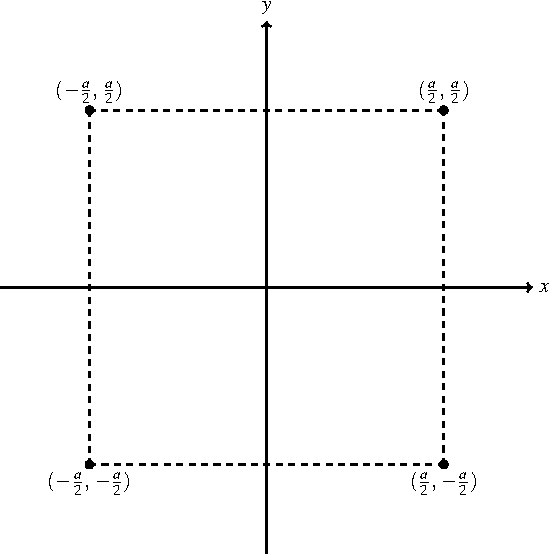
\includegraphics[scale=1.1]{image/03/square.pdf}
  \caption{%%
  }
  \label{fig:square_four_corners}
  \end{figure}
  \end{solution}
}{}

\item You move the square from \Problem{prob:square_centre_origin} by
  $b \geq 0$ units to the right and $b$ units upward.  Determine the
  new coordinates of each of the four corners of the square and the
  new coordinates of the centre of the square.
\ifbool{showSolution}{
  \begin{solution}
  See \Figure{fig:square_shifted}.
  %%
  \begin{figure}[!htbp]
  \centering
  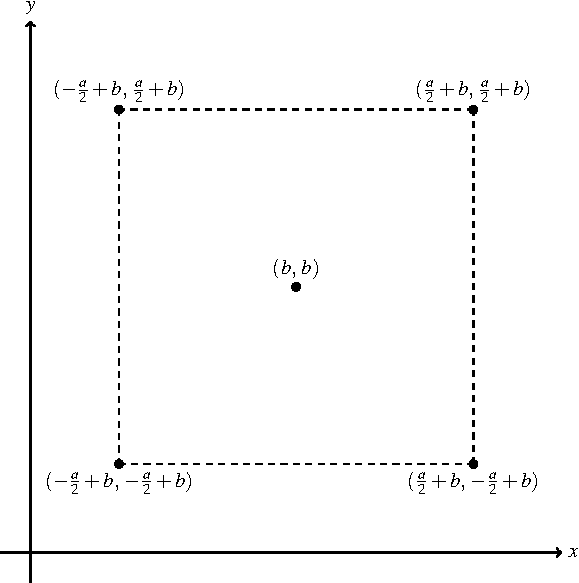
\includegraphics[scale=1.1]{image/03/square-shifted.pdf}
  \caption{%%
    The square from \Problem{prob:square_centre_origin} shifted by
    $b \geq 0$ units to the right and $b$ units upward.  The four
    corners of the square and the centre are shifted by $b$ units
    horizontally and vertically.
  }
  \label{fig:square_shifted}
  \end{figure}
  \end{solution}
}{}

\item Each side of a triangle has a length of one unit.  You draw the
  triangle in the Cartesian coordinate system.  Calculate the
  coordinates of each of the three corners of the triangle.
\ifbool{showSolution}{
  \begin{solution}
  Let $a \geq 0$ and $b \geq 0$ be real numbers.  You can draw the
  triangle in such a way that its base is on the $x$-axis with the
  middle of the base being the origin.  So two corner points of the
  triangle lie on the $x$-axis.  Let those corner points be
  $\tuple{a}{0}$ and $\tuple{-a}{0}$.  The third point is the
  coordinates $\tuple{0}{b}$.  Since the base is one unit, the
  distance from $\tuple{a}{0}$ to the origin must be $1 / 2$.  The
  distance from $\tuple{-a}{0}$ to the origin is also $1 / 2$ and so
  the length of the base is $\frac{1}{2} + \frac{1}{2} = 1$ unit.  In
  other words, the value of $a$ is $a = 1 / 2$.  The three corners of
  the triangle are $(-\frac{1}{2}\comma 0)$, $(\frac{1}{2}\comma 0)$,
  and $\tuple{0}{b}$.

  Let's now calculate the value of $b$.  Note that the points
  $\tuple{0}{0}$, $(\frac{1}{2}\comma 0)$, and $\tuple{0}{b}$ form
  the corners of a right-angled triangle.  The distance from
  $(\frac{1}{2}\comma 0)$ to the origin is $1 / 2$ and so the
  right-angled triangle has a base of $1 / 2$ units.  The height of
  the triangle is $b$ and the hypotenuse is one unit.  Now use
  Pythagoras' theorem to write
  \[
  \parenthesis*{\frac{1}{2}}^2 + b^2
  =
  1^2.
  \]
  Solve the last equation for $b^2$ to get
  %%
  \begin{align*}
  b^2
  &=
  1 - \frac{1}{4} \\[4pt]
  &=
  \frac{3}{4}.
  \end{align*}
  %%
  Solve the latter equation for $b$ to get
  %%
  \begin{align*}
  b
  &=
  \sqrt{\frac{3}{4}} \\[4pt]
  &=
  \frac{\sqrt{3}}{\sqrt{4}} \\[4pt]
  &=
  \frac{\sqrt{3}}{2}.
  \end{align*}
  %%
  Therefore the three points $(-\frac{1}{2}\comma 0)$,
  $(\frac{1}{2}\comma 0)$, and $(0\comma \frac{\sqrt{3}}{2})$ are the
  corners of a triangle each of whose sides has a length of one unit.
  See \Figure{fig:unit_triangle}.

  \begin{figure}[!htbp]
  \centering
  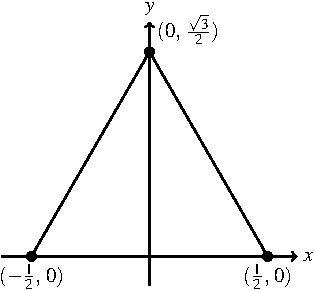
\includegraphics[scale=1.1]{image/03/unit-triangle.pdf}
  \caption{%%
    The three corners of a triangle.  Each side of the triangle has a
    length of one unit.
  }
  \label{fig:unit_triangle}
  \end{figure}
  \end{solution}
}{}

\item Let $a > 0$ be a real number.  An ant starts at the point
  $\tuple{a}{0}$ in the Cartesian coordinate system and moves in a
  straight line to the point $\tuple{a}{a}$.  From $\tuple{a}{a}$ the
  ant moves in a straight line to $\tuple{0}{a}$.  The ant then moves
  in a straight line to its starting position.  If the ant travelled a
  total distance of $d$, explain why the total distance is
  \[
  d
  =
  a(2 + \sqrt{2}).
  \]
\ifbool{showSolution}{
  \begin{solution}
  The distance from $\tuple{a}{0}$ to $\tuple{a}{a}$ is
  %%
  \begin{align*}
  \sqrt{
    (a - 0)^2 + (a - a)^2
  }
  &=
  \sqrt{a^2 + 0^2} \\[4pt]
  &=
  \sqrt{a^2} \\[4pt]
  &=
  a.
  \end{align*}
  %%
  The distance from $\tuple{a}{a}$ to $\tuple{0}{a}$ is
  %%
  \begin{align*}
  \sqrt{
    (a - a)^2 + (0 - a)^2
  }
  &=
  \sqrt{0^2 + (-a)^2} \\[4pt]
  &=
  \sqrt{(-1)^2 \times a^2} \\[4pt]
  &=
  \sqrt{a^2} \\[4pt]
  &=
  a.
  \end{align*}
  %%
  The distance from $\tuple{0}{a}$ to $\tuple{a}{0}$ is
  %%
  \begin{align*}
  \sqrt{
    (0 - a)^2 + (a - 0)^2
  }
  &=
  \sqrt{(-a)^2 + a^2} \\[4pt]
  &=
  \sqrt{(-1)^2 \times a^2 + a^2} \\[4pt]
  &=
  \sqrt{a^2 + a^2} \\[4pt]
  &=
  \sqrt{2a^2} \\[4pt]
  &=
  \sqrt{2} \times \sqrt{a^2} \\[4pt]
  &=
  a\sqrt{2}.
  \end{align*}
  %%
  The total distance that the ant travelled is
  %%
  \begin{align*}
  a + a + a\sqrt{2}
  &=
  2a + a\sqrt{2} \\[4pt]
  &=
  a(2 + \sqrt{2}).
  \end{align*}
  \end{solution}
}{}

\item Let $a > 0$ be a real number.  An ant starts at the origin and
  moves in a straight line to the point $\tuple{a}{a}$.  The ant then
  moves in a straight line to its starting position.  Explain why the
  total distance that the ant travelled is $2a\sqrt{2}$.
\ifbool{showSolution}{
  \begin{solution}
  The distance from $\tuple{0}{0}$ to $\tuple{a}{a}$ is
  %%
  \begin{align*}
  \sqrt{
    (a - 0)^2 + (a - 0)^2
  }
  &=
  \sqrt{a^2 + a^2} \\[4pt]
  &=
  \sqrt{2a^2} \\[4pt]
  &=
  a\sqrt{2}.
  \end{align*}
  %%
  Since the ant then returns to its starting position, the total
  distance travelled is twice the distance $a\sqrt{2}$.  Therefore the
  ant travelled a total distance of $2a\sqrt{2}$.
  \end{solution}
}{}

\item Read about chess on Wikipedia or elsewhere on the Internet.
  \begin{packedenum}
  \item\label{subprob:chessboard}
    Draw the chessboard.  Label its horizontal and vertical
    coordinates.

  \item\label{subprob:chessboard_coordinate_system}
    Explain the coordinate system that is used to name each of the
    $64$ squares of a chessboard.
  \end{packedenum}
\ifbool{showSolution}{
\begin{solution}
\solutionpart{subprob:chessboard}
See \Figure{fig:empty_chessboard}.

\solutionpart{subprob:chessboard_coordinate_system}
Chess uses a coordinate system to name each of the $64$ squares of a
chessboard.  Starting from the bottom of the board and going to the
top, the rows are numbered as $\seq{1}{2}{8}$.  Starting from the left
of the board and going to the right, the columns are labelled as
$\seq{{\rm a}}{{\rm b}}{{\rm h}}$.  To specify a square of the
chessboard, you write the column name followed by the row number.  For
example, in \Figure{fig:chessboard_queen_knight} the queen is at the
square d4 and the knight is at the square g7.

\begin{figure}[!htbp]
\centering
\subfigure[]{
  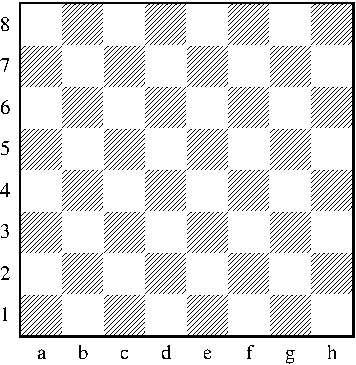
\includegraphics[scale=1]{image/03/chessboard.pdf}
  \label{fig:empty_chessboard}
}
%%
\qquad
%%
\subfigure[]{
  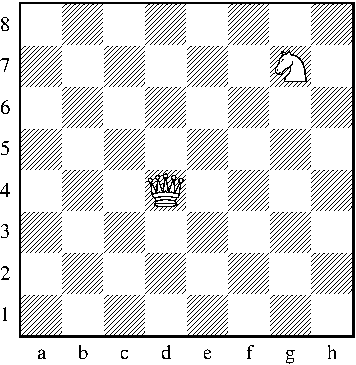
\includegraphics[scale=1]{image/03/chessboard-pieces.pdf}
  \label{fig:chessboard_queen_knight}
}
\caption{%%
  Two $8 \times 8$ chessboards.
}
\label{fig:chessboard}
\end{figure}
\end{solution}
}{}
\end{problem}

\end{document}
